\documentclass{beamer}

\usepackage[utf8]{inputenc}
\usepackage[francais]{babel}
\usepackage{wrapfig}
\usepackage{amsmath}% http://ctan.org/pkg/amsmath

\usepackage{sansmathaccent}
\pdfmapfile{+sansmathaccent.map}
\usepackage{tikz}
\usepackage{verbatim}

\usetheme{Singapore}

\title{Détection d'anomalies de classification dans l'IoT via Machine Learning}
\author{Antoine Urban, Yohan Chalier}
\institute{Projet de filière SR2I \\ Télécom ParisTech}

\begin{document}

\begin{frame}
\titlepage
\end{frame}

\begin{frame}
  \frametitle{Introduction}
La détection d'obstacles: un enjeu de sécurité! \\
\bigskip
\begin{figure}[b]
\centering
\includegraphics[width=0.6\textwidth]{img/sensors.png}
\caption{Ensemble des capteurs présents dans le véhicule\label{sensors}}
\end{figure}


\end{frame}

\begin{frame}
  \frametitle{Attaques potentielles}
  
\begin{description}\setlength{\itemsep}{1.5mm}
\item[Attaque par aveuglement des capteurs]

\begin{figure}
\includegraphics[scale=0.2,right]{img/blinding.png}
\end{figure}

\item[Attaque par modification]

\begin{figure}
\flushright
\includegraphics[scale=0.3,right]{img/data_flow.png}
\end{figure}

\end{description}

\end{frame}


\begin{frame}
  \frametitle{Objectifs}

\begin{block}{ }
Proposition d'un modèle de classification multi-classes en réalisant un classeur à partir d’un algorithme d’apprentissage supervisé
\end{block}

\begin{figure}
\centering
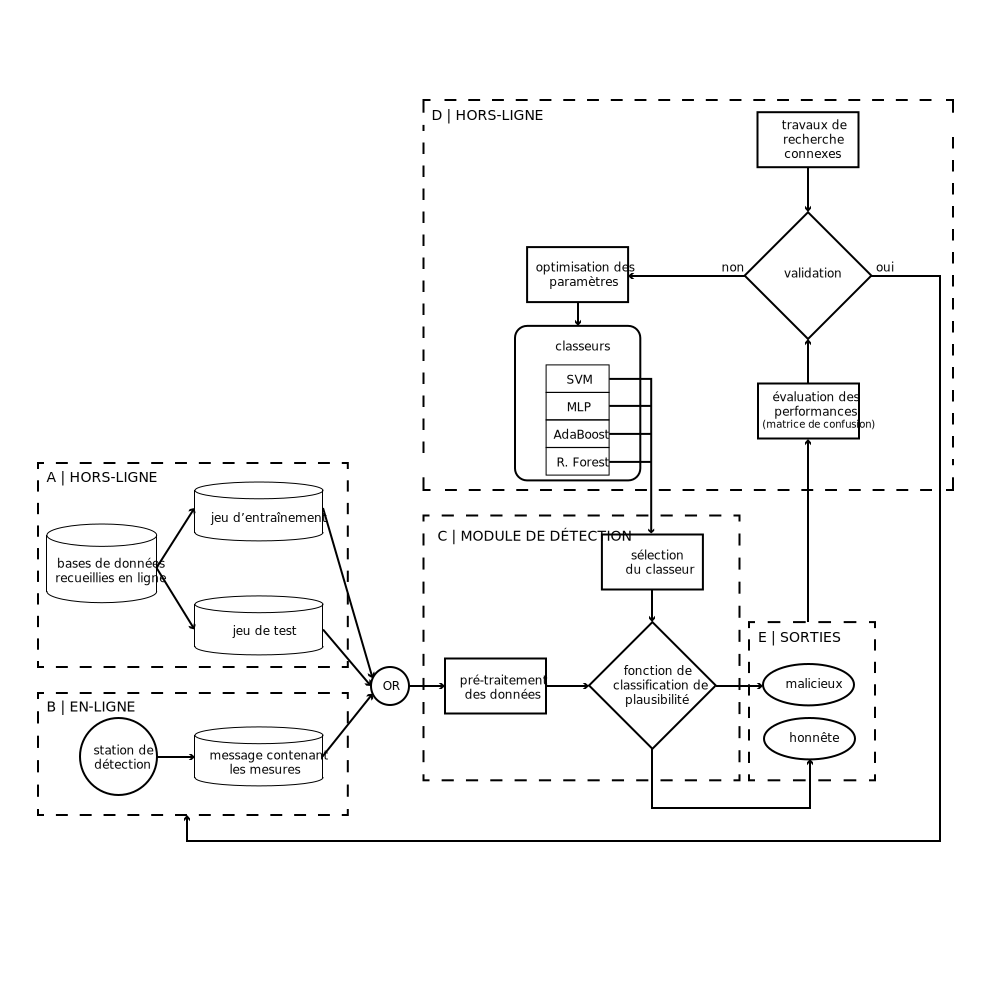
\includegraphics[width=0.75\textwidth]{img/structure.png}

\end{figure}

\end{frame}

\begin{frame}
  \frametitle{Méthodes d'évaluation }
\medskip
\framesubtitle{\begin{LARGE}
Matrice de confusion
\end{LARGE}}

\begin{tabular}{ l | l | c | c | c c}
\multicolumn{2}{c}{} & \multicolumn{2}{c}{Classe réelle} & \\
\cline{3-4}
\multicolumn{2}{c|}{} & Positif & Négatif \\
\cline{2-4}
\multirow{2}{*}{Classe prédite} & Positif & $TP$ & $FP$ & $PPV$ & $FDR$ \\
\cline{2-4}
& Négatif & $FN$ & $TN$ & $FOR$ & $NPV$ \\
\cline{2-4}
\multicolumn{1}{r}{} & \multicolumn{1}{l}{} & \multicolumn{1}{c}{$TPR$} & \multicolumn{1}{c}{$FPR$} \\
\multicolumn{1}{l}{} & \multicolumn{1}{l}{} & \multicolumn{1}{c}{$FNR$} & \multicolumn{1}{c}{$TNR$} \\
\end{tabular}

\end{frame}

\begin{frame}
  \frametitle{Méthodes d'évaluation}
\medskip
\framesubtitle{\begin{LARGE}
Score F1
\end{LARGE}}

\begin{block}{ }
\textbf{Objectif:}Maximisation du score F1 comme critère de performance
\end{block}

\begin{equation}
	\text{f1-score} = \dfrac{2\times(\text{Recall} \times \text{Precision})}{(\text{Recall} + \text{Precision})} = 2\times\dfrac{PPV \times TPR}{PPV + TPR}
\end{equation}

\bigskip
\bigskip

\begin{equation}
\text{Precision} = \dfrac{TP}{TP+FP}
\end{equation}\\
\begin{equation}
\text{Recall} = \dfrac{TP}{TP+FN}
\end{equation}


\end{frame}

\end{document}